\documentclass[fleqn]{article}

\usepackage{graphicx}
\usepackage{xurl}
\usepackage{url}
\usepackage{caption}
\usepackage{fancyhdr}
\usepackage{mathtools}
\usepackage{amsmath}
\usepackage{amssymb}
\usepackage{tikz}
\usepackage{listings}
\usepackage{xcolor}
\usepackage{float}

\definecolor{codegreen}{rgb}{0,0.6,0}
\definecolor{codegray}{rgb}{0.5,0.5,0.5}
\definecolor{codepurple}{rgb}{0.58,0,0.82}
\definecolor{backcolour}{rgb}{0.95,0.95,0.92}

\lstdefinestyle{mystyle}{
    backgroundcolor=\color{backcolour},   
    commentstyle=\color{codegreen},
    keywordstyle=\color{magenta},
    numberstyle=\tiny\color{codegray},
    stringstyle=\color{codepurple},
    basicstyle=\ttfamily\footnotesize,
    breakatwhitespace=false,         
    breaklines=true,                 
    captionpos=b,                    
    keepspaces=true,                 
    numbers=left,                    
    numbersep=5pt,                  
    showspaces=false,                
    showstringspaces=false,
    showtabs=false,                  
    tabsize=2
}

\lstset{style=mystyle}

\usepackage{xepersian}

\settextfont[BoldFont={XB Zar bold.ttf}]{XB Zar.ttf}
\setlength\parindent{0pt}



\newcommand{\expnumber}{پنچم}



\title{

\includegraphics[width=0.4\textwidth]{sharif.png}\\
\normalsize{دانشکده مهندسی کامپیوتر}\\
\vspace{1cm}
    
\huge{آزمایشگاه معماری کامپیوتر}
\\ \vspace{.8cm}
\Large{گزارش آزمایش \expnumber}
\\ \vspace{.8cm}
\Large{عنوان آزمایش : واحد محاسبه با امکان انتخاب ثبات مبدا و مقصد}
}

\author{
\\
دکتر حمید سربازی آزاد
\\ \vspace{.4cm}
\\
  سارا آذرنوش       ---      98170668
\\ \vspace{0.2cm} \\
  کسری امانی       ---      98101171
\\ \vspace{0.2cm} \\
  پارسا محمدیان       ---      98102284
\\ \vspace{.4cm}
}

\date{\today}

\begin{document}

\clearpage\maketitle
\thispagestyle{empty}

\newpage

\pagestyle{fancy}
\lhead{آزمایشگاه معماری کامپیوتر}

\rhead{آزمایش \expnumber}

\tableofcontents

\setcounter{page}{1}

\newpage

\section{مقدمه}
کامپیوترهای امروزی از بخش‌های مختلفی تشکیل شدند که یکی از بخش‌های اصلی آن‌ها 
\lr{CPU (Central Processing Unit)} 
است که مسئول پردازش است. یکی از بخش‌های اصلی و جدا نشدنی واحد پردازنده مرکزی، 
\lr{ALU (Arithmetic and Logic Unit)}
است. همانطور که از اسم واحد محاسبه و منطق مشخص است، پردازش‌های محاسباتی در واحد پردازنده مرکزی 
بر عهده این بخش می‌باشد. ورودی‌های واحد محاسبات با توجه به معماری پردازنده تعیین می‌شوند. 
برای نمونه پردازنده‌های تک عملونده، دو عملونده، و سه عملونده، داریم که عدد موجود در هر کدام تعداد عملوندهای 
\lr{Explicit}
یا صریح را مشخص می‌کند. در مقابل عملوند 
\lr{Implicit}
یا ضمنی در دستور ماشین مشخص نمی‌شود و به صورت پیشفرض در نظر گرفته شده است مانند ماشین انباشتگر یا 
\lr{Accumulator} 
که در آن یک ثبات در نظر گرفته می‌شود و به عنوان مقصد، و یکی از مبداهای محاسبات استفاده می‌شود. 
حال اگر به شکل 
\ref{arch}
نگاه کنیم، معماری واحد محاسبات به گونه‌ای است که یکی از عملوندهای مبدا به صورت ضمنی 
\lr{$R_0$}
است و دیگر عملوند مبدا و عملوند مقصد به صورت صریح مشخص می‌شوند. در ادامه مشاهده می‌کنیم 
که در این معماری سه عملوند 
\lr{Immediate} 
نیز وجود دارد. این اعداد، اعداد پرکاربردی هستن که به دلیل کاربرد فراوانشان به صورت 
غیرقابل تغییر در مدار موجود هستند. همچنین 
\lr{Multiplexer} 
موجود یک ورودی دیگر دارد که در این آزمایش استفاده نمی‌شود ولی بعدها برای 
\lr{Flag}
استفاده می‌شود. 
\lr{Flag}ها 
مجموعه بیت‌هایی هستند که پس از پایان عملیات حسابی بر اساس نتیجه عملیات پر می‌شوند. 
این پرچم‌ها معمولا شامل موارد زیر هستند : 
\begin{enumerate}
  \item C : Carry
  \item Z : Zero
  \item S : Sign
  \item O : Overflow
\end{enumerate}

\begin{figure}[!htbp]
  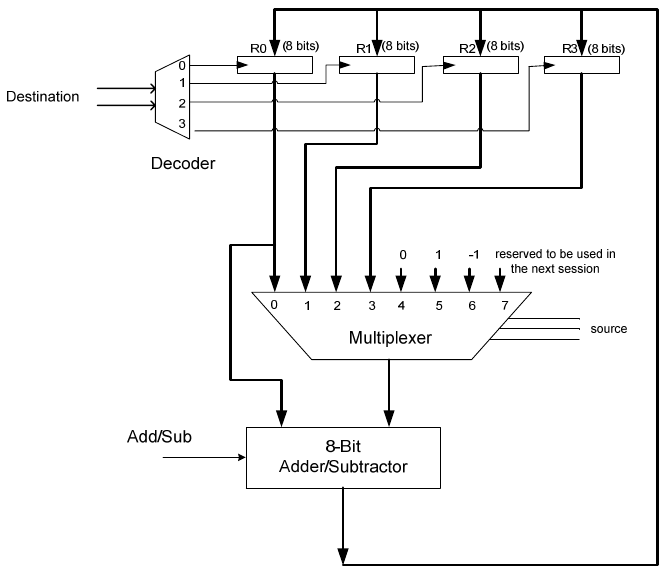
\includegraphics[width=\textwidth]{Assets/architecture.png}
  \caption{معماری واحد محاسبات}
  \label{arch}
\end{figure}

\section{هدف آزمایش}
در این آزمایش قصد داریم بخشی از یک کامپیوتر ساده را طراحی کنیم. این بخش شامل یک 
\lr{Register File} 
که درون خود دارای 4 ثبات 8 بیتی است، 
و یک 
\lr{ALU (Arithmetic and Logic Unit)} 
که عملگرهای جمع و تفریق را دارد، است. برای طراحی و پیاده‌سازی این بخش از نرم‌افزار 
\lr{Proteus}
استفاده می‌کنیم. 

\section{قطعات مورد نیاز}
قطعات مورد استفاده در این آزمایش در زیر آمده اند : 

\begin{itemize}
  \item گیت \lr{XOR}
  \item گیت \lr{NOT}
  \item گیت \lr{OR}
  \item گیت \lr{AND}
  \item \lr{LOGICPROBE}
  \item \lr{LOGICPROBE (BIG)}
  \item \lr{LOGICSTATE}
  \item \lr{SWITCH}
  \item \lr{BUTTON}
  \item \lr{74S139 IC $\rightarrow$ 2 to 4 Decoder}
  \item \lr{74198 IC $\rightarrow$ 8-Bit Register}
  \item \lr{3WATT10K Resistor}
  \item \lr{74157 $\rightarrow$ Quadruple 1-of-2 Multiplexer}
\end{itemize}

\section{شرح آزمایش}

همانطور که گفته شد قسمت محاسباتی یک 
\lr{CPU}
ساده را طراحی می‌کنیم. برای ساخت مدار از طراحی موجود در شکل 
\ref{arch}
استفاده می‌کنیم. این معماری امکان انجام جمع و تفریق با انتخاب یکی از ثبات‌های‌ مبدا و ثبات 
نگهدارنده نتیجه (مقصد) را دارد.

\subsection{قالب فرمان‌های واحد محاسبات}

دستورات این واحد محاسبات 6 بیتی هستند و فرمت دستورات در شکل 
\ref{command}
آمده است. 

\begin{figure}[!htbp]
  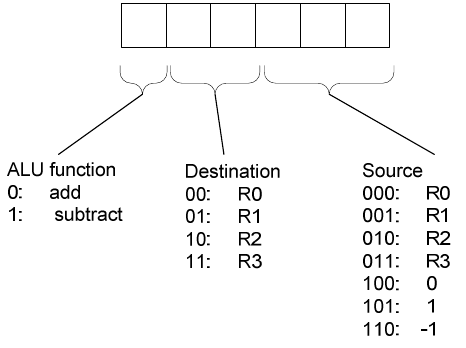
\includegraphics[width=\textwidth]{Assets/commands.png}
  \caption{فرمت دستورات واحد محاسبه}
  \label{command}
\end{figure}

عملوندها در 4 رجیستر 8 بیتی 
\lr{$R_0$}
تا 
\lr{$R_3$}
قرار دارند.
مقدار هر یک از رجیسترها به یک 
\lr{Multiplexer}
با 8 ورودی 8 بیتی وارد می‌شود که با توجه به سه بیت آخر دستور ورودی مناسب به خروجی وصل می‌شود و وارد 
\lr{َAdder/Subtractor}
می‌گردد. همچنین ورودی دیگر آن نیز به صورت ضمنی ثبات 
\lr{$R_0$}
است.

با توجه به بیت اول دستور، نوع عملیات (جمع/تفریق) مشخص می‌گردد (اگر 0 باشد جمع و اگر 1 باشد تفریق است).

خروجی 
\lr{Adder/Subtractor}
به همه ثبات‌ها متصل است. پایه‌ی لود کردن موازی ثبات مطلوب به وسیله یک 
\lr{Decoder}
و توسط دو بیت وسط دستور فعال می‌گردد و در نهایت نتیجه محاسبات در آن دخیره می‌شود.

\subsection{طراحی \lr{Adder/Subtractor}}

با توجه به 8 بیتی بودن اعداد نیاز به یک جمع/تفریق کننده 8 بیتی داریم. برای ساخت آن مانند آزمایش قبل عمل می‌کنیم.
یک جمع کننده کامل 
(\lr{Full Adder})
با گیت های پایه می‌سازیم. مدار تمام جمع‌کننده در شکل 
\ref{fa}
آمده است.

\begin{figure}[!htbp]
  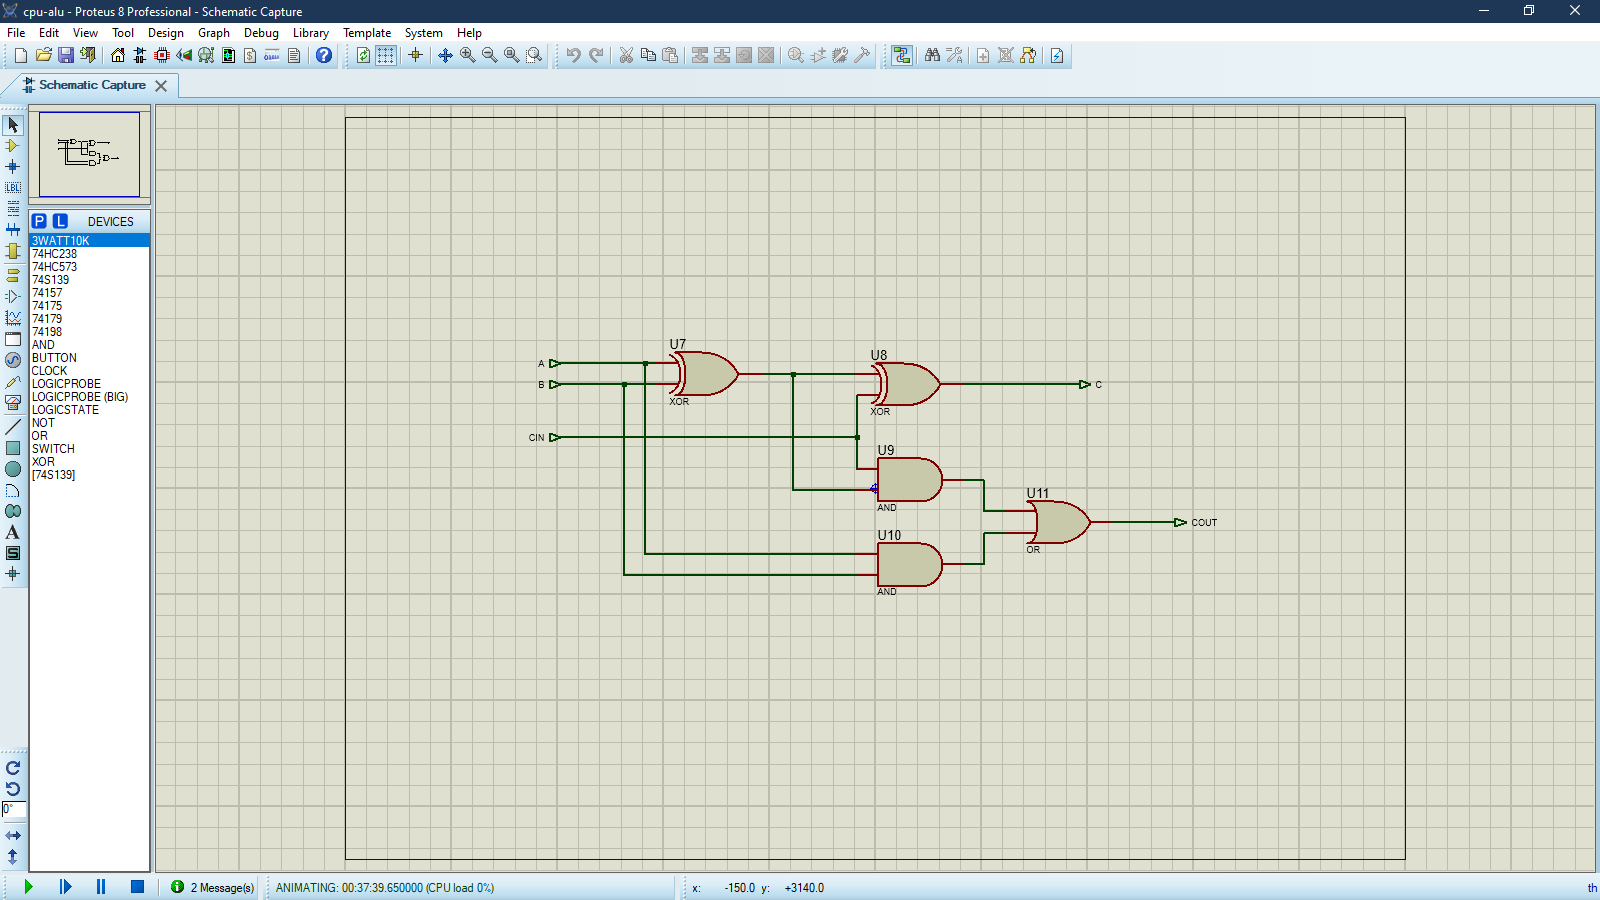
\includegraphics[width=\textwidth]{Assets/fa.png}
  \caption{مدار تمام جمع‌کننده}
  \label{fa}
\end{figure}
 
سپس با استفاده از 8 جمع کننده کامل و اتصال متوالی آن‌ها می‌توانیم 
\lr{Ripple-Carry Adder}
بسازیم. می‌دانیم عملیات تفریق در مبنای دو همان عملیات جمع با مکمل 2 یک عدد است. 
پس برای اضافه کردن عملیات تفریق، یک بیت عملیات به عنوان ورودی ماژول در نظر می‌گیریم، 
در صورتی که 1 بود تمام بیت‌های عدد دوم را معکوس می‌کنیم و کل عدد را با یک جمع می‌کنیم. 
عملیات معکوس کردن 8 بیت عدد دوم با استفاده از 8 گیت 
\lr{XOR} 
انجام شده است و عملیات جمع کردن با یک، با پاس دادن رقم نقلی اولیه انجام شده است. 
به این صورت هر وقت 
\lr{func} 
یک باشد عملیات تفریق (جمع با مکمل دو) انجام می‌شود. مدار این جمع/تفریق کننده در شکل 
\ref{as}
قابل مشاهده است. 

\begin{figure}[!htbp]
  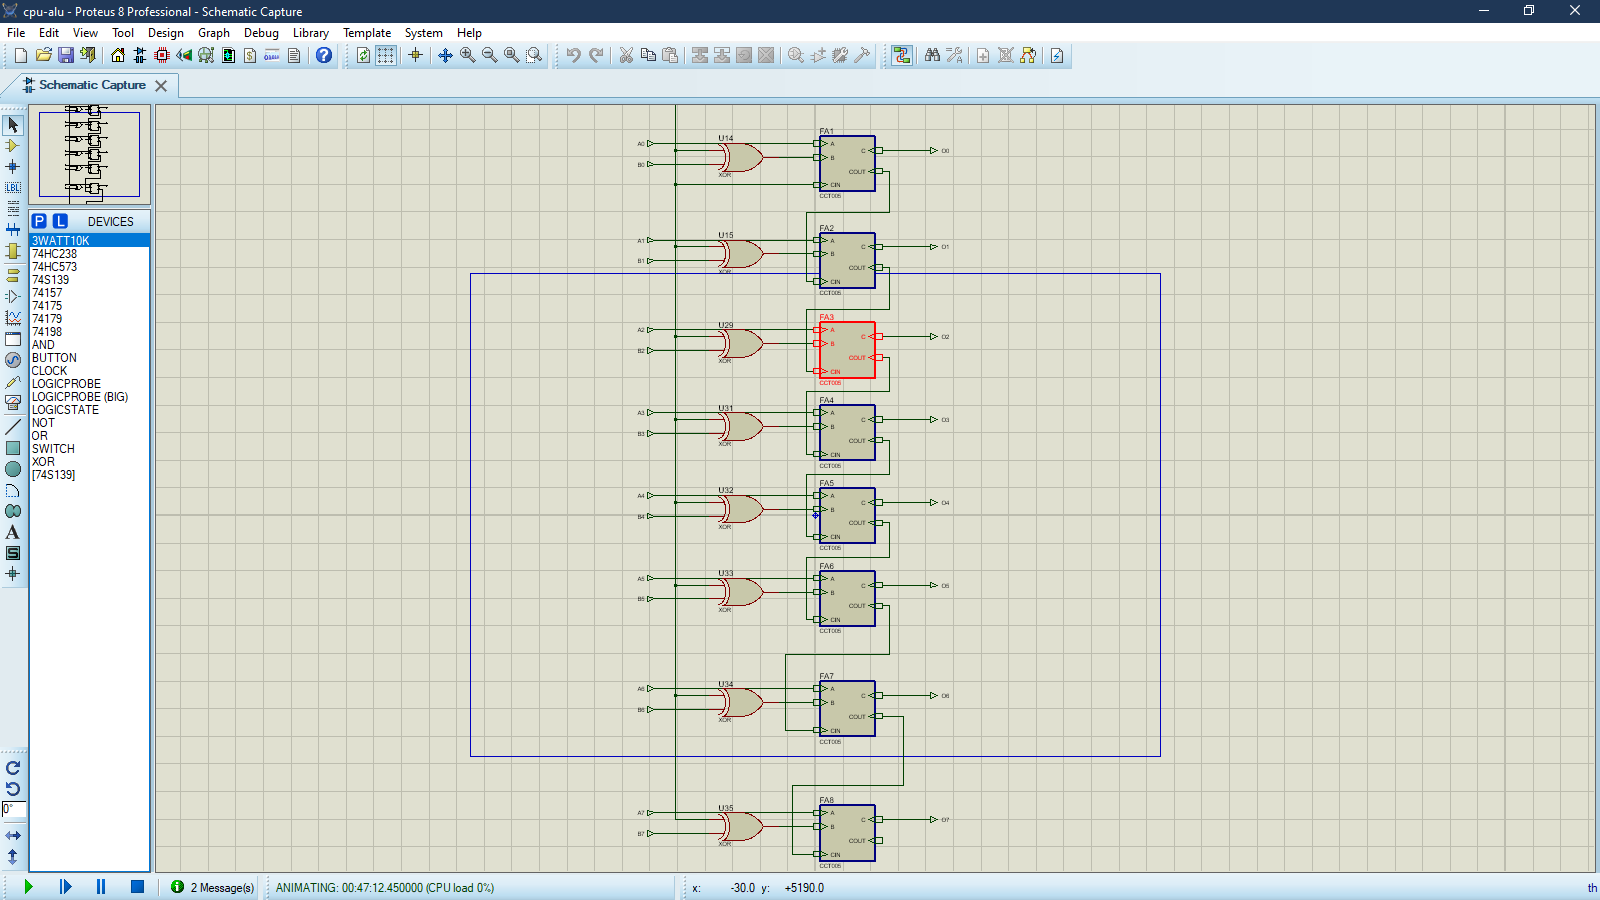
\includegraphics[width=\textwidth]{Assets/as.png}
  \caption{مدار جمع‌/تفریق کننده}
  \label{as}
\end{figure}

\subsection{طراحی مولتی‌پلکسر با 8 ورودی 8 بیتی}

برای ساختن مولتی‌پلکسر با 8 ورودی 8 بیتی، ابتدا ماژول مولتی‌پلکسری با 2 ورودی 8 بیتی می‌سازیم. 
این ماژول با استفاده از دو آی سی 
\lr{74157} 
ساخته شده است. پیاده‌سازی مدار این ماژول را در شکل 
\ref{mux_inner}
مشاهده می‌کنیم. 

\begin{figure}[!htbp]
  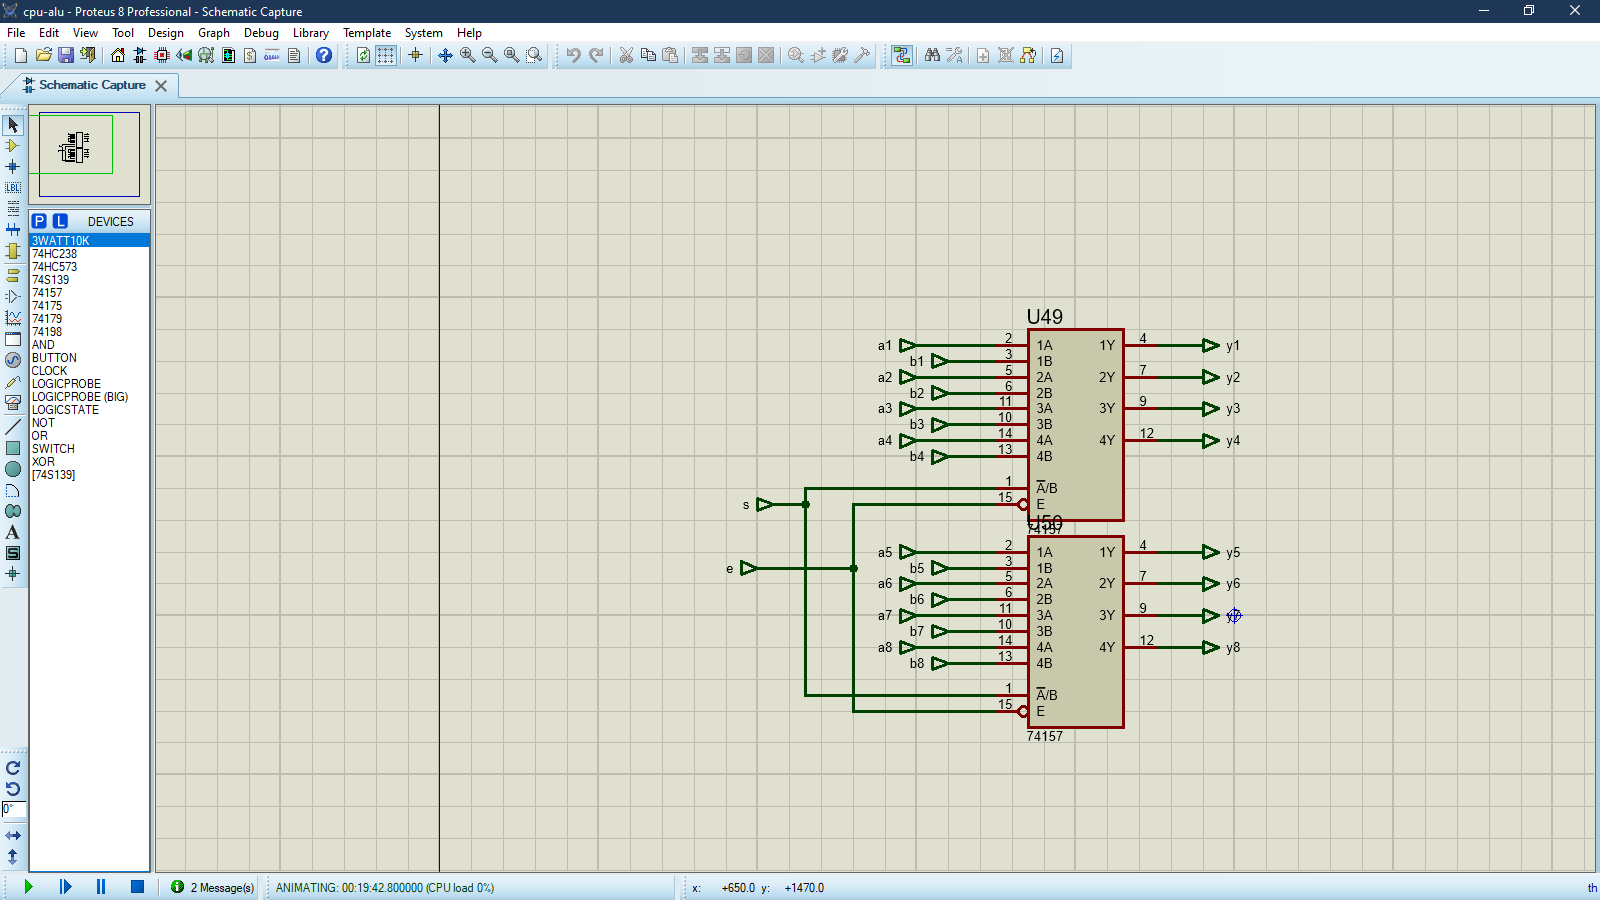
\includegraphics[width=\textwidth]{Assets/mux_inner.png}
  \caption{مدار درونی مولتی‌پلکسر}
  \label{mux_inner}
\end{figure}

حال هفت عدد از ماژول ساخته شده را متوالی وصل می‌کنیم تا مولتی‌پلکسر مطلوب را بسازیم. این اتصال به گونه‌ای است 
که از 3 لایه ماژول ساخته شده تشکیل شده است. لایه اول بیت 
\lr{$S_0$} 
به ماژول‌ها داده می‌شود، 
لایه دوم بیت 
\lr{$S_1$}
و لایه آخر بیت 
\lr{$S_2$}. 
مدار نهایی این ماژول نیز در شکل 
\ref{mux}
قابل مشاهده است. 

\begin{figure}[!htbp]
  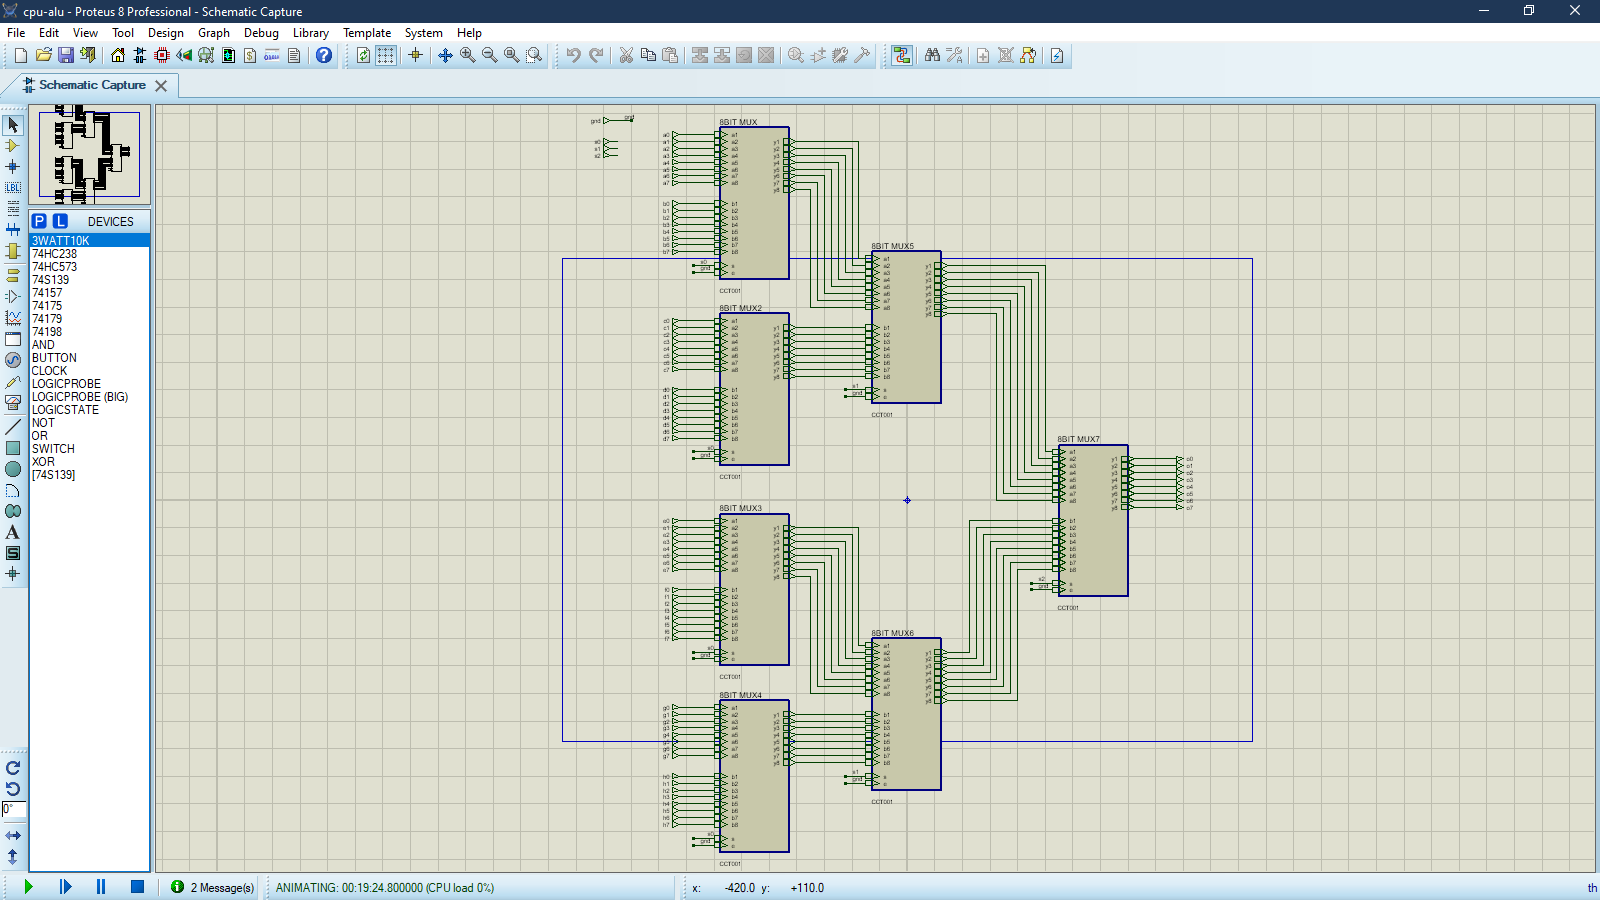
\includegraphics[width=\textwidth]{Assets/mux.png}
  \caption{مدار مولتی‌پلکسر}
  \label{mux}
\end{figure}

\subsection{کلید \lr{Enable}}

مدار با بستن کلید 
\lr{Enable}
فعال می‌شود و یا توجه به دستور داده شده، شروع به کار می‌کند. کلید 
\lr{Enable}
از یک سمت به مقاومت و مقدار 1، و از سمت دیگر به زمین متصل است. با بستن کلید چون به زمین وصل می‌شود مقدار آن 0 می‌شود و با استفاده از نات آن مقدار 
\lr{Enable}
یک می‌شود و مدار فعال می‌شود. 
دقت شود که این سیگنال در پردازنده نیاز نیست و صرفا برای انجام تست اضافه شده است. چون در پردازنده در هر سیکل ساعت 
پردازش انجام می‌شود.

\section{نتیجه آزمایش}

در آخر مدار یک واحد محاسبات را داریم که قابلیت انتخاب ثبات یکی از ورودی‌ها و خروجی را دارد. مدار نهایی 
در شکل 
\ref{final}
قابل مشاهده است. 

\begin{figure}[!htbp]
  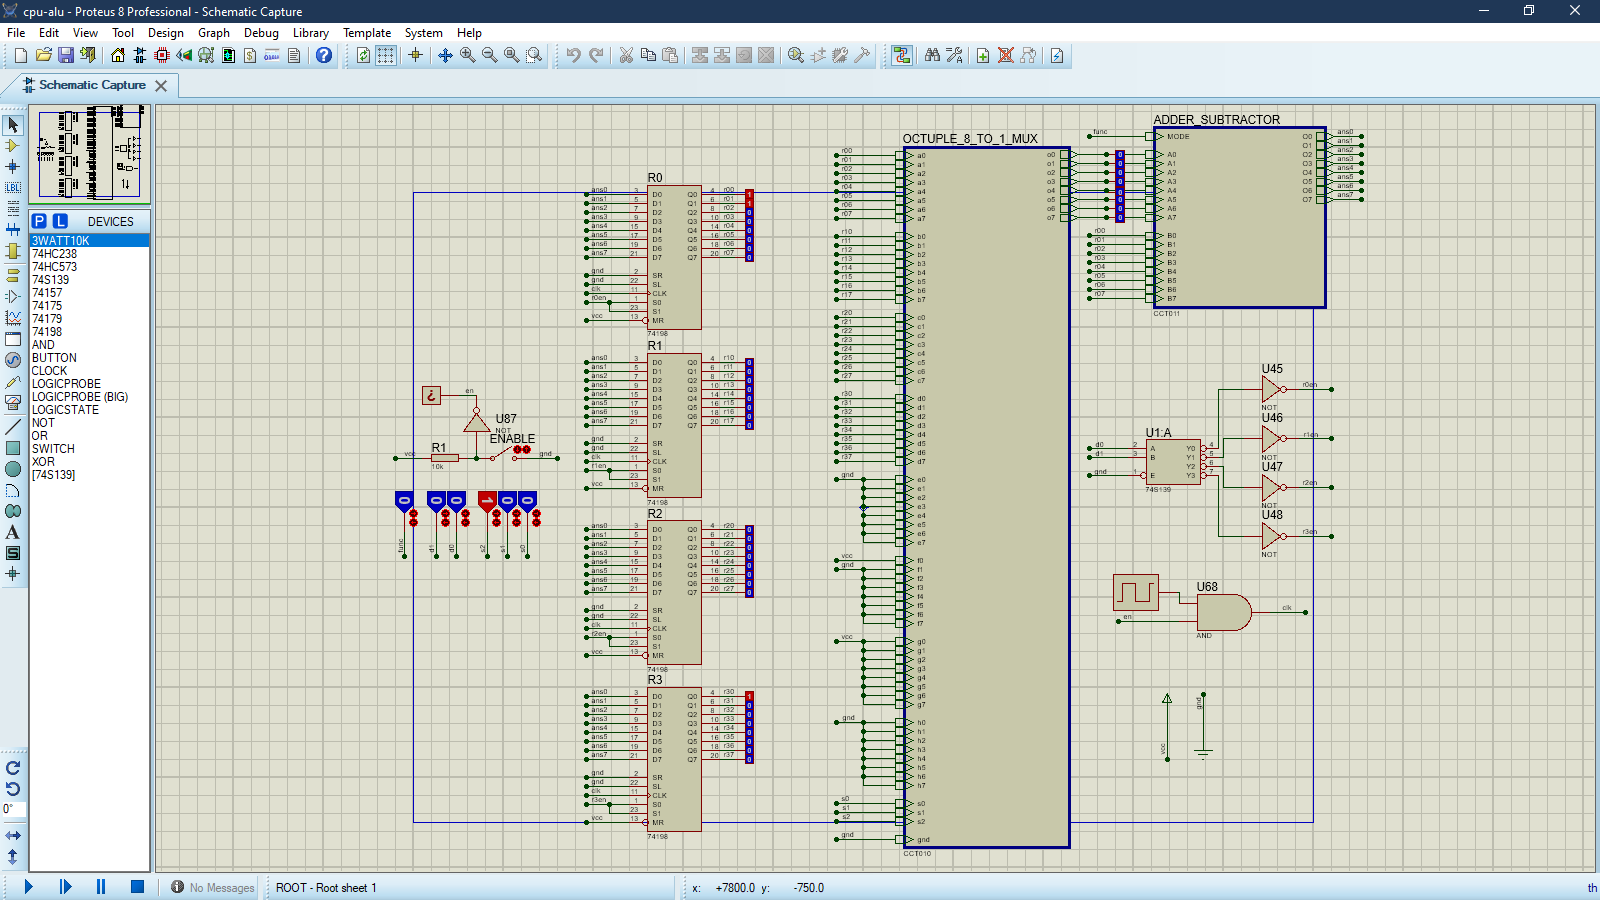
\includegraphics[width=\textwidth]{Assets/final.png}
  \caption{مدار نهایی}
  \label{final}
\end{figure}

برای تست مدار چندین ورودی مختلف را تست می‌کنیم. 

\subsection{تست}

در این تست ابتدا دو بار 
\lr{$R_0 = R_0 + 1$}
انجام شده که در شکل 
\ref{t1}
و
\ref{t2}
قابل مشاهد است. سپس 
\lr{$R_0 = R_0 + R_0$}
انجام شده است که در شکل 
\ref{t3}
قابل مشاهده است. پس از آن 
\lr{$R_1 = R_0 + R_0$}
انجام شده است که در شکل 
\ref{t4}
نمایان است. بعد از آن 
\lr{$R_2 = R_0 + R_0$}
اجرا شده است که در شکل 
\ref{t5}
مشخص است. سپس 
\lr{$R_3 = R_1 + R_0$}
اجرا شده است که در شکل 
\ref{t6}
آمده است. 
در آخر برای اطمینان از صحت عملگر تفریق 
\lr{$R_3 = R_3 - R_0$}
اجرا شده است که در شکل 
\ref{t7}
نتیجه مشاهده می‌شود. 

\begin{figure}[!htbp]
  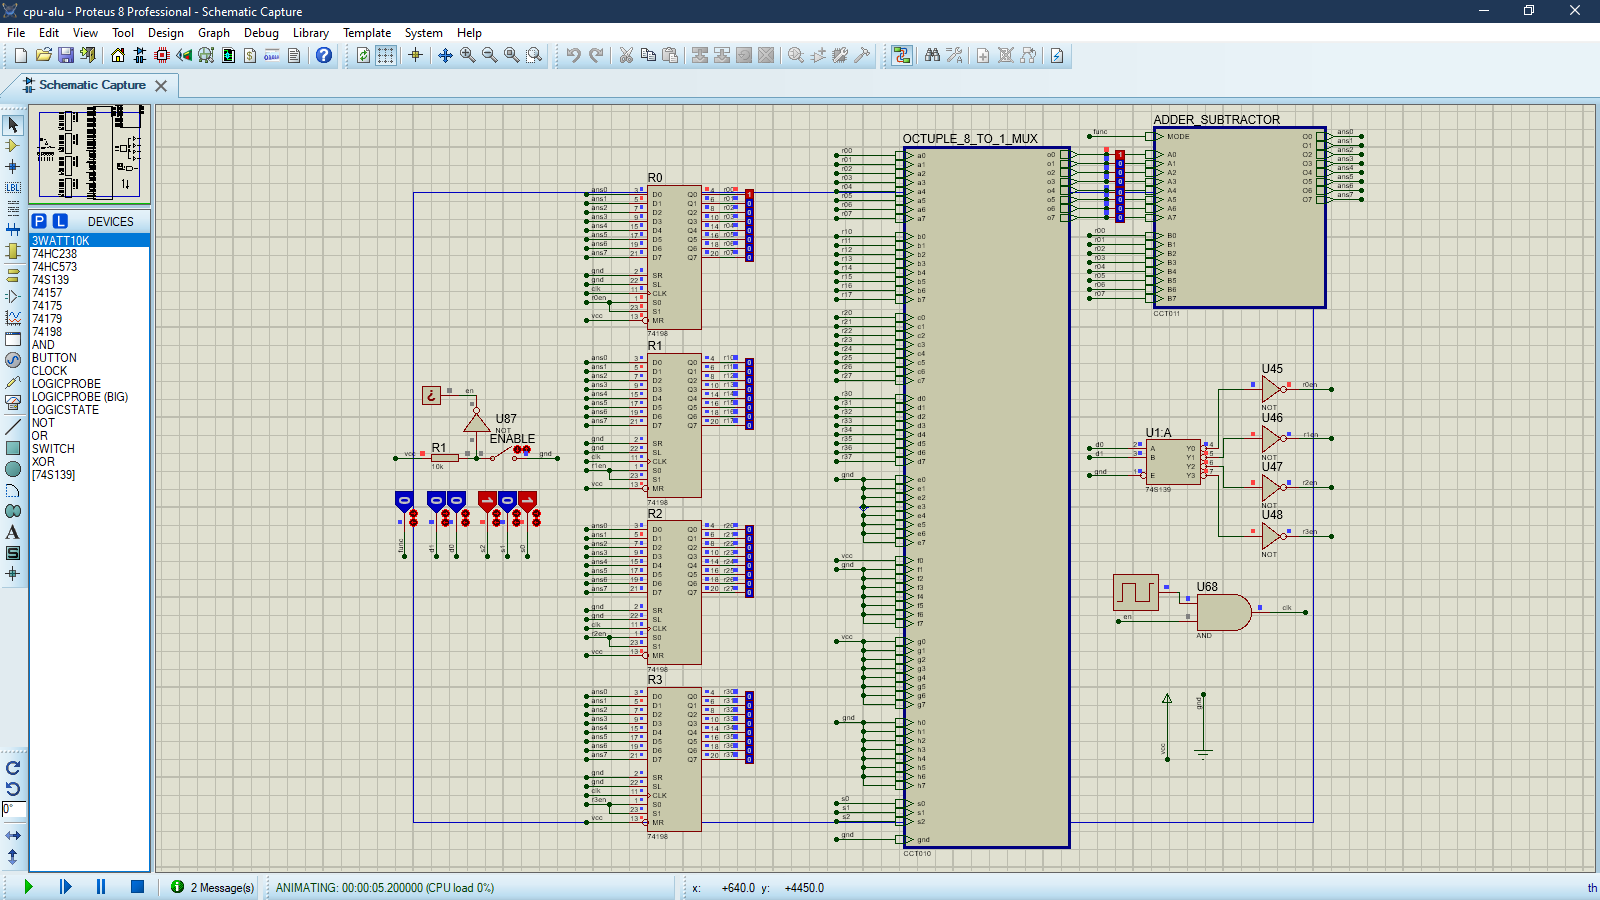
\includegraphics[width=\textwidth]{Assets/t1.png}
  \caption{}
  \label{t1}
\end{figure}

\begin{figure}[!htbp]
  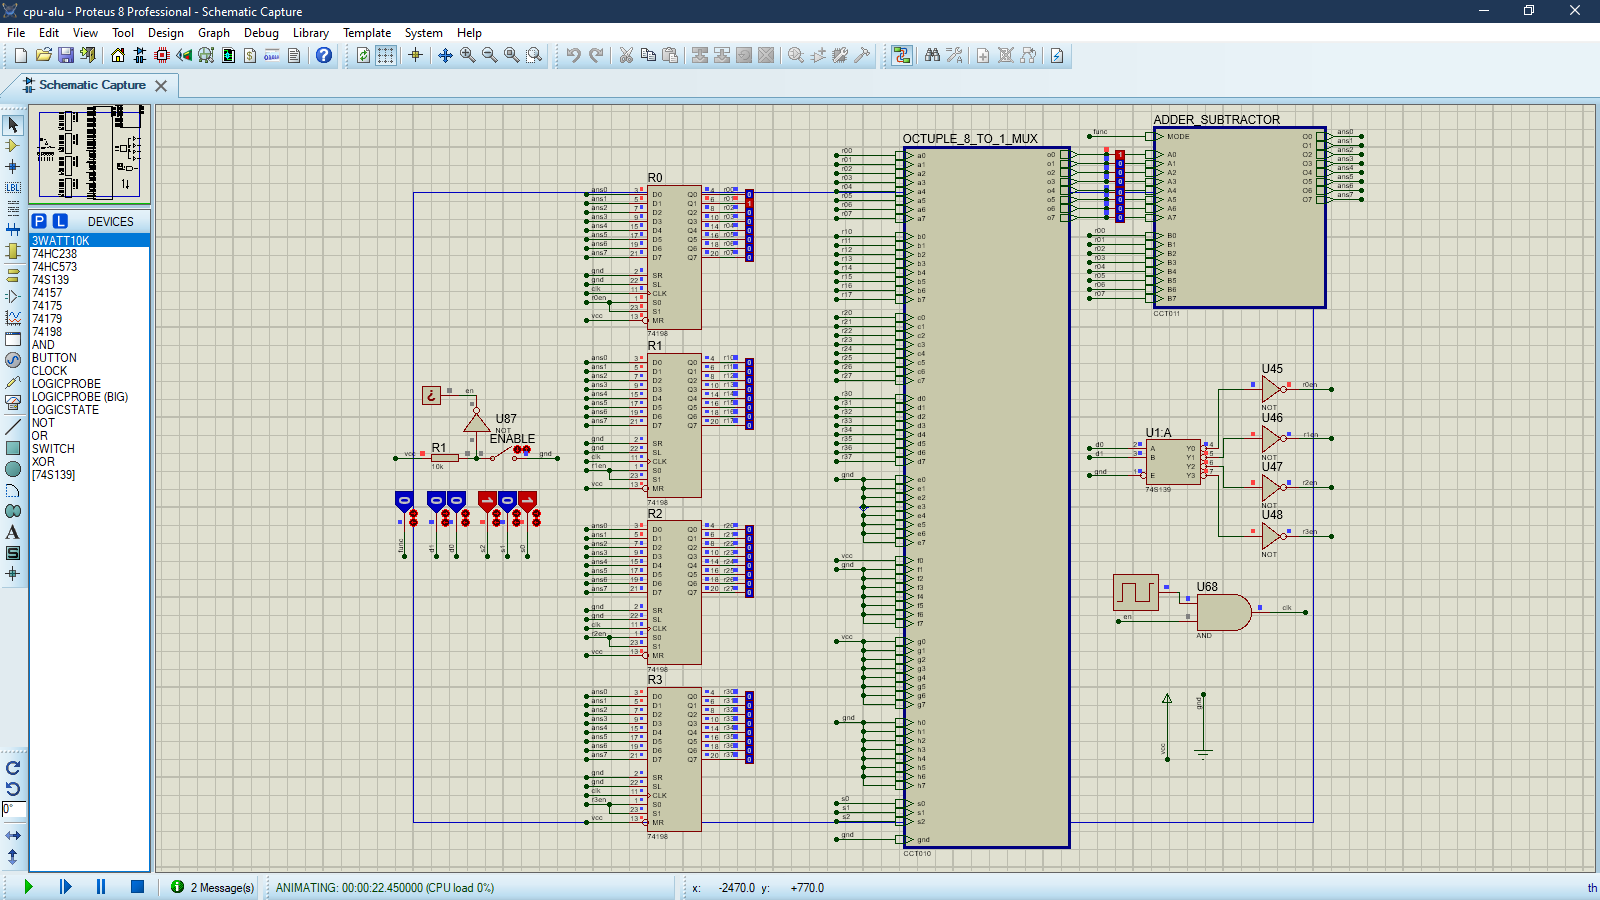
\includegraphics[width=\textwidth]{Assets/t2.png}
  \caption{}
  \label{t2}
\end{figure}

\begin{figure}[!htbp]
  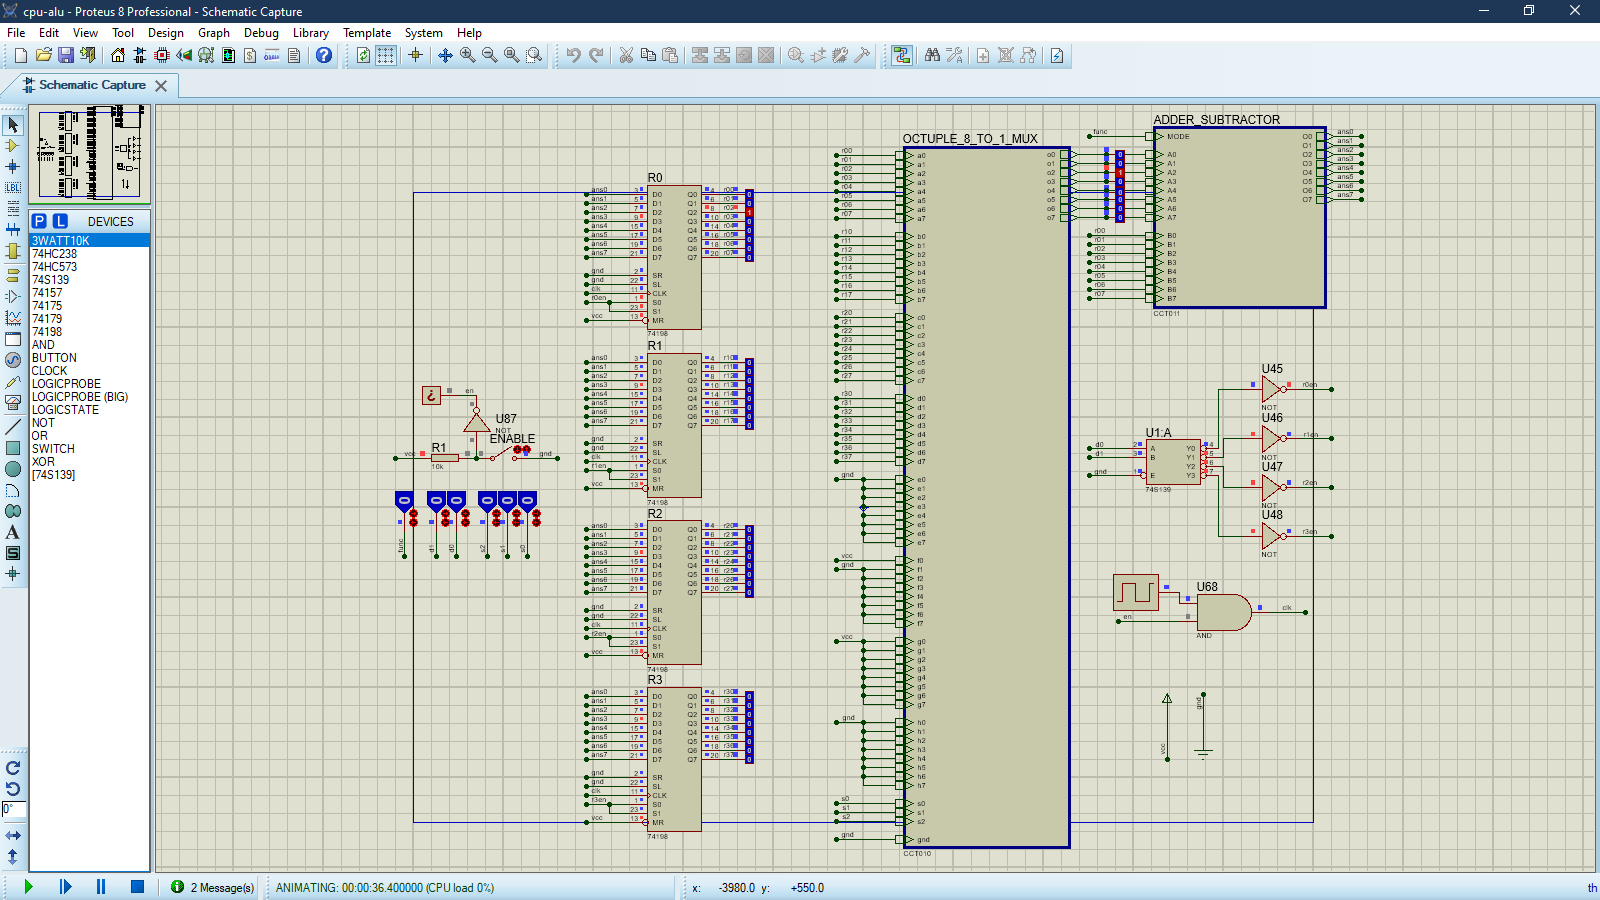
\includegraphics[width=\textwidth]{Assets/t3.png}
  \caption{}
  \label{t3}
\end{figure}

\begin{figure}[!htbp]
  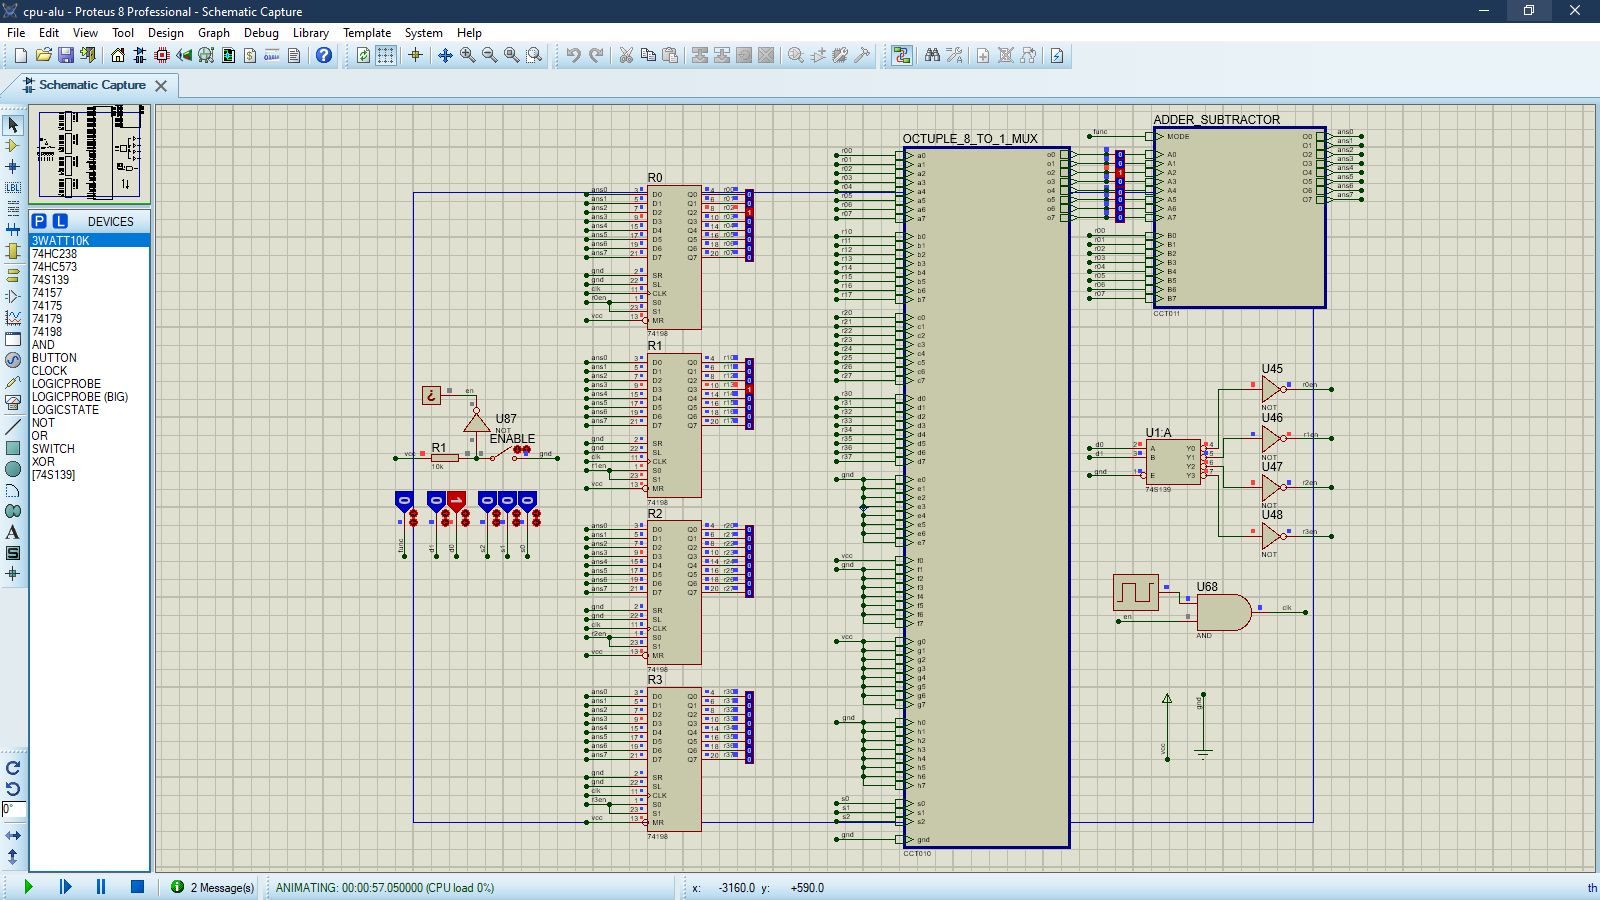
\includegraphics[width=\textwidth]{Assets/t4.png}
  \caption{}
  \label{t4}
\end{figure}

\begin{figure}[!htbp]
  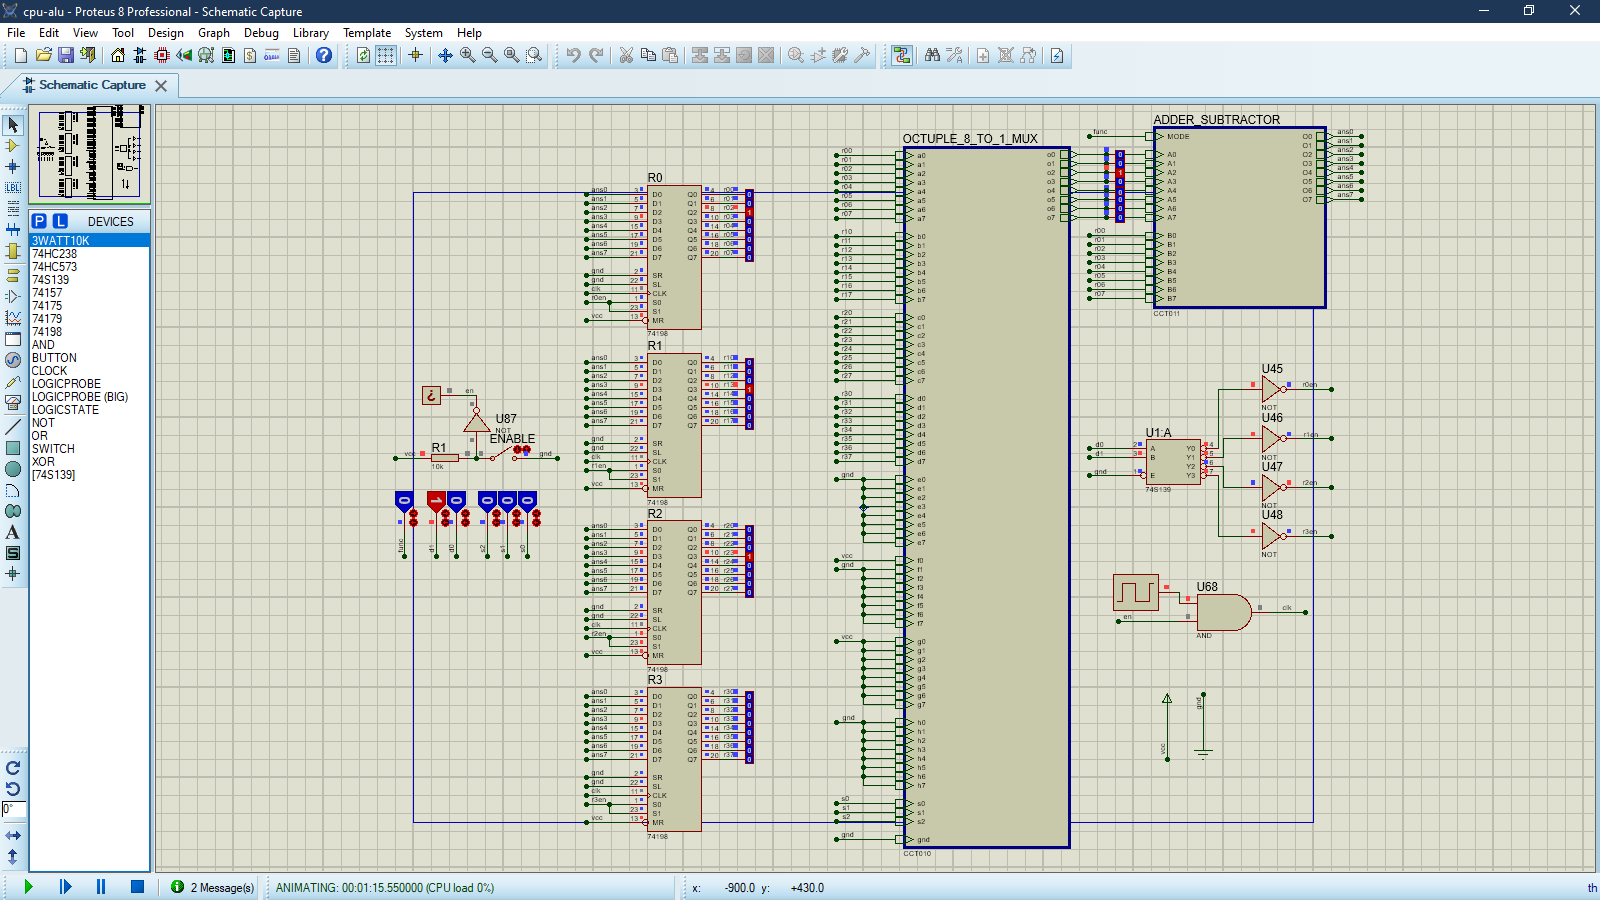
\includegraphics[width=\textwidth]{Assets/t5.png}
  \caption{}
  \label{t5}
\end{figure}

\begin{figure}[!htbp]
  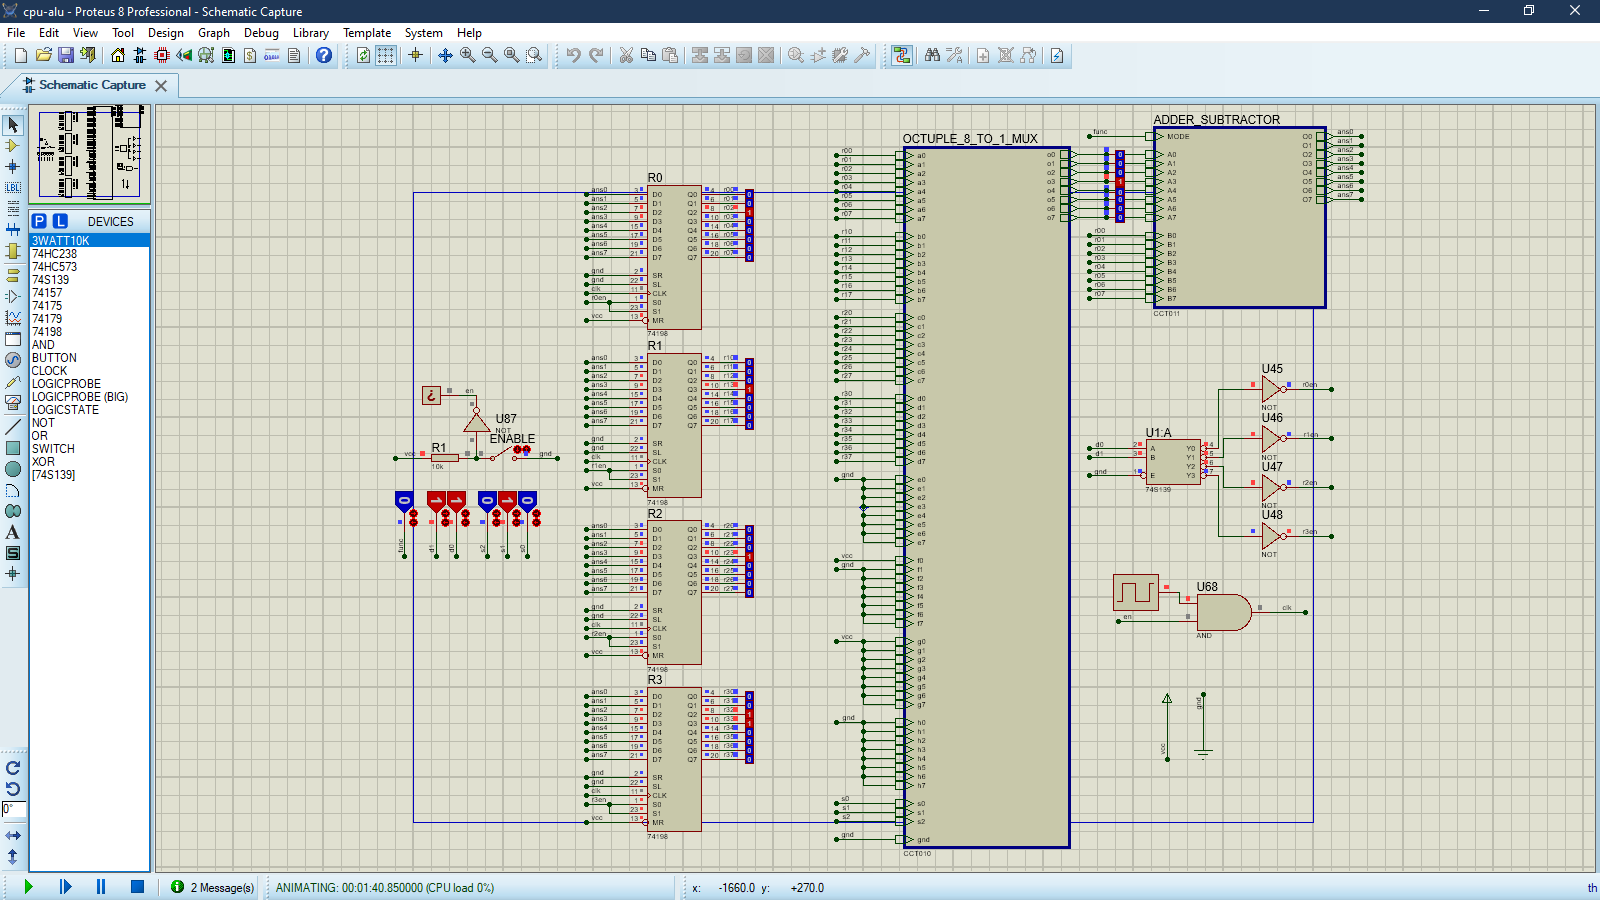
\includegraphics[width=\textwidth]{Assets/t6.png}
  \caption{}
  \label{t6}
\end{figure}

\begin{figure}[!htbp]
  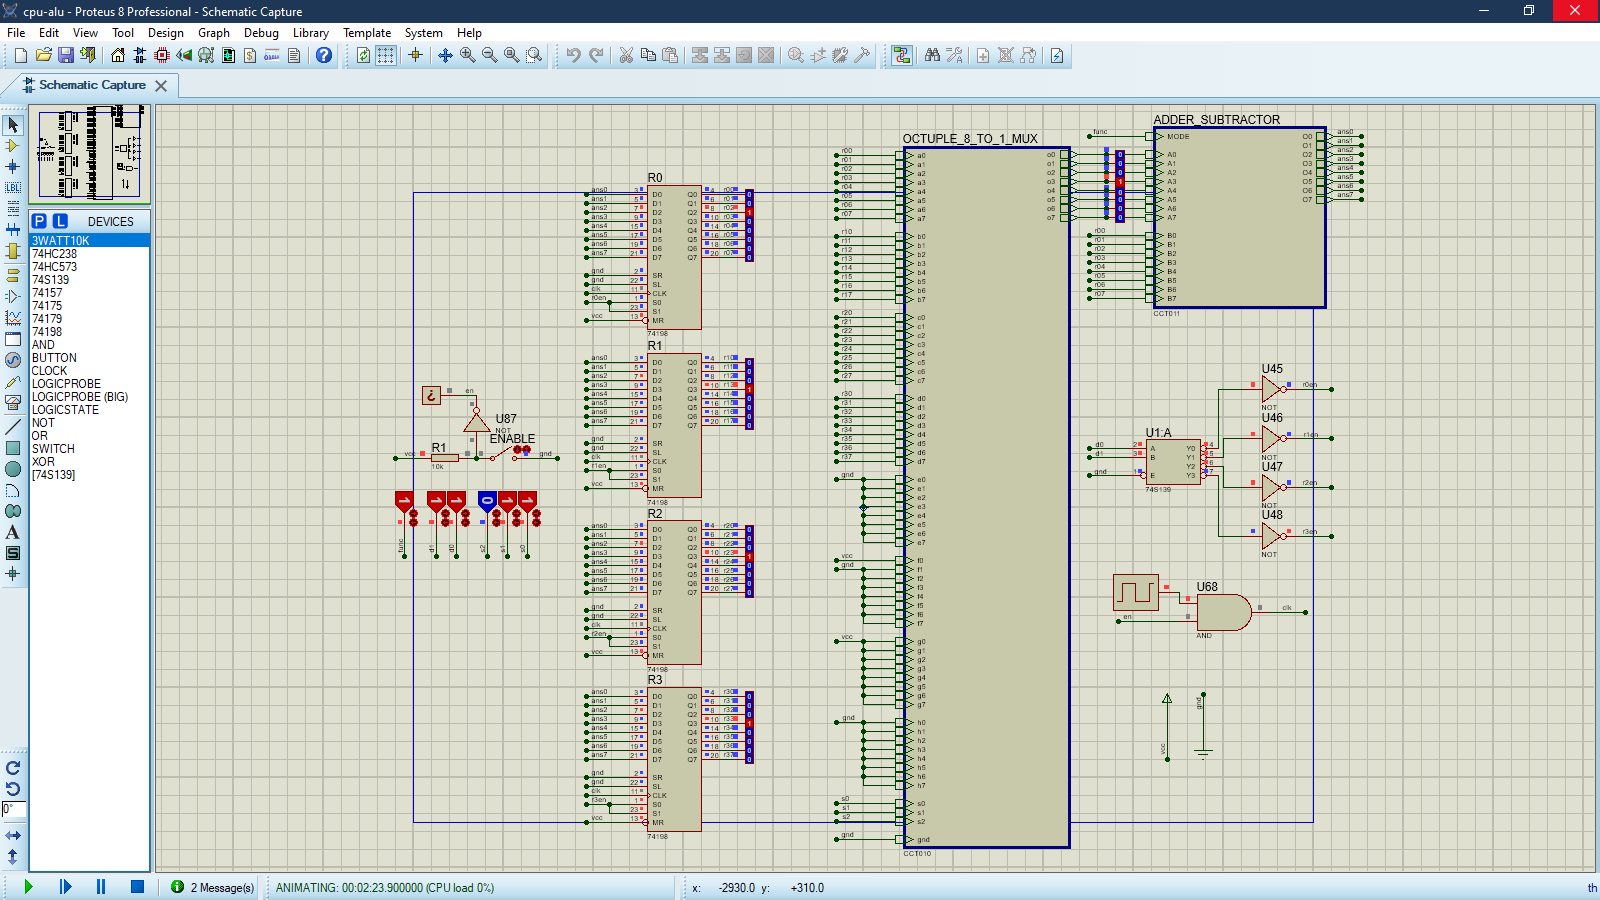
\includegraphics[width=\textwidth]{Assets/t7.png}
  \caption{}
  \label{t7}
\end{figure}
\end{document}
